The most popular 3D modeling toolbox is most-probably OpenCascade \cite{OpenCascade}, which also offers a voxelizer. Nonetheless, due to its size and cumbersome installation requirements on for example a linux system, we decided to also look for different open source software. We found a library which we employed for voxelization, called CVMLCPP.


The \emph{Common Versatile Multi-purpose Library for C++} (CVMLCPP) is a collection of mathematical algorithms whose objective is "to eliminate this redundancy by offering high-quality implementations of commonly needed functionality" \cite{CVMLCPP}. The library offers an easy-to-use voxelizer, which we use for conversion of CAD input to a boolean voxel grid.

\begin{figure}
\centering
\begin{subfigure}{
  
\includegraphics[width=.2\linewidth]{Pictures/STLToVoxels/Star_STL.png}}
\end{subfigure}
\begin{subfigure}{
  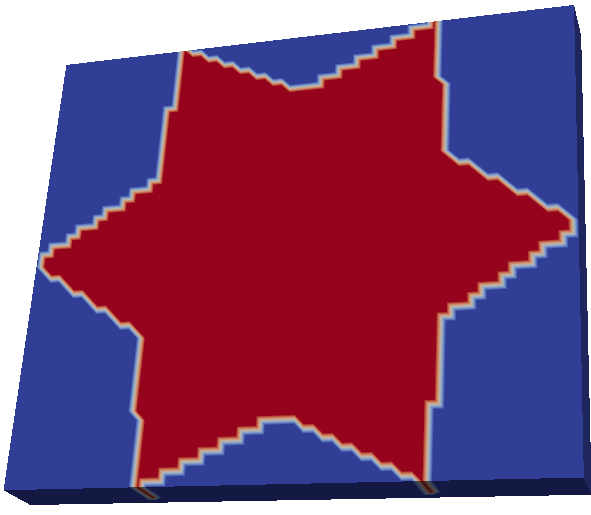
\includegraphics[width=.2\linewidth]{Pictures/STLToVoxels/Star_VTK_Trans.png}}
\end{subfigure}
\caption{The STL geometry of a star (left) and its voxelized form (right) obtained via the CVMLCPP voxelizer, visualized by Paraview \cite{Paraview}.}
\label{fig: voxelizerStar}
\end{figure}

In terms of implementation, we first had to install the CVMLCPP library. Next, since the library is open source, we adapted the voxelizer to our needs. %In the end, to voxelize a file given as .stl-input, we could just call 
%\begin{lstlisting}
%~/Path/To/CVMLCPP/bin/voxelize ./<stl_file>.stl <voxelSize>
%\end{lstlisting}
%where $\mathtt{<voxelSize>}$ is an integer declaring the size of a voxel. 
The output gets written to a .dat binary file. An example result of using the voxelizer is illustrated in \autoref{fig: voxelizerStar}.